While Commuting Zones are thought of as representing local labor markets, they have a number of shortcomings for empirical research that are not regularly discussed in the literature. In this section, we evaluate the sensitivity of Commuting Zone definitions for two aspects of the TS1996 methodology. First, the method is highly sensitive to variation in the input data, and if the input data are measured with error, the definitions may convey a false sense of certainty. Second, the resulting clusters are very sensitive to the decision of when to stop merging clusters, which implies that small changes in the chosen cutoff height drastically affect the number and size of clusters. Overall, this uncertainty in the definition of commuting zones contributes to conventional standard errors understating the true level of uncertainty in estimates, as well as non-classical measurement error that may bias empirical estimates. At the end of the section, we list other weaknesses that also undermine commuting zones as a definition of local labor markets.

\subsection{Sensitivity of Clustering Results to Underlying Error}
Given the reliance of TS1996 on the commuting flows data, we want to analyze the extent to which the outputs of the TS1996 methodology are sensitive to error in the input data. First, recall equation \ref{eqn:distance} for the dissimilarity matrix entries. If $f_{ij}$ is measured without error, then $D_{ij}$ is measured without error. However, if the flows are measure with some error, $\epsilon_{ij}$, then we have an estimate of $D_{ij}$, $\hat{D}_{ij}$, which can be expressed as below:
\begin{equation}
\hat{D}_{ij} = 1- \hat{P}_{ij} = 1- \frac{f_{ij}+\epsilon_{ij} + f_{ji} + \epsilon_{ji}}{\min(\hat{rlf}_i,\hat{rlf}_j)}
\end{equation}	
Now suppose without loss of generality that county $i$ is the smaller county; that means that 
\[
\hat{D}_{ij} =1- \frac{f_{ij}+\epsilon_{ij} + f_{ji} + \epsilon_{ji}}{ rlf_i + \sum_j \epsilon_{ij}}
\]
Or, rewritten:
\[
\hat{D}_{ij} =1- \frac{f_{ij} + f_{ji} }{rlf_i + \sum_j \epsilon_{ij}}+\frac{\epsilon_{ij} + \epsilon_{ji}}{ rlf_i + \sum_j \epsilon_{ij}}
\]
However, even if $E[\sum_j \epsilon_{ij}]=0$, we only have one realization of this draw (the published figures), which were calculated from survey responses. Additionally, we know two things about $\epsilon_{ij}$. First, $\epsilon_{ij} / f_{ij}$ is larger for smaller counties. Second, this implies that $rlf_i$ is 
more subject to measurement error for small counties than larger counties.
This will increase $D_{ij}$ for some small counties and decrease it for others. Because of the hierarchical nature of the clustering method, this will affect the formation of all other clusters in the data.\footnote{Additionally, because the heights are normalized in the procedure, it also affects where the effective cutoff is, even for counties unaffected by errors in flows.}

To demonstrate how this measurement error affects the outcome of the clustering procedure, we use journey-to-work data from the pooled 2009-2013 ACS because it has published margins of error (hereafter, MOEs).\footnote{In the 2009-2013 ACS, the average ratio of margin of error to reported commuting flow (unweighted) is 1.24. The Decennial Census numbers do not publish margins of error, but presumably they are somewhat smaller than ACS MOEs. Later in the paper, we use the 2009-2013 ACS MOEs to estimate the MOEs for the 1990 JTW flows.} For reference, summary statistics on the ratio of the margins of error to the flows are in Table \ref{tab:moesum} in the appendix, and show that margins of error are much larger relative to smaller flows. Using these MOEs, we perform the following analysis: 

\begin{enumerate}
	\item For each origin-destination pair, we draw $\epsilon_{ij}$ from a normal distribution
 with mean 0 and standard deviation $MOE_{ij}/(2 \times 1.64)$, since the MOE is the 90\% confidence interval.
	\item Add the value from (1) to the reported flow ($\hat{f}_{ij} = f_{ij} + \epsilon_{ij}$).
	\item Re-aggregate the flows, recalculate the dissimilarity matrix, and re-run the TS1996 clustering procedure.
	\item Using the new clusters, calculate the following statistics: average number of counties in a cluster; the number of clusters; and the total number of counties in a different cluster than the one they would have been assigned, had the flows been assigned using only the published flow estimates (that is, not taking into account the MOE).
\end{enumerate}
%
% Source program: module_perturbjtw2009.sas
% Last updated:

\begin{figure}[th]
\caption{Sensitivity Analysis}
%\begin{subfigure}
\begin{tabular}{ccc}
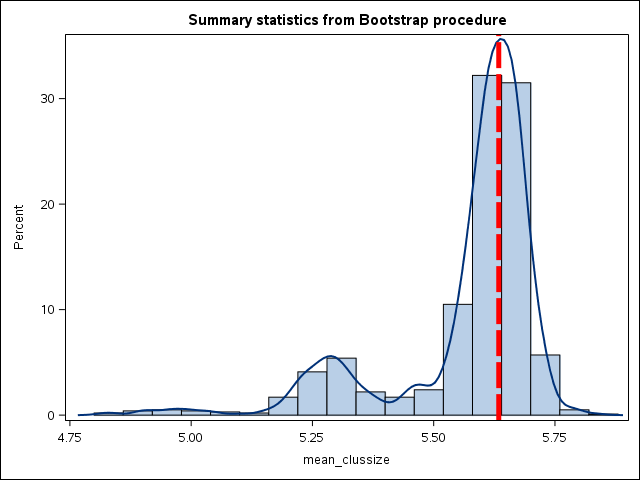
\includegraphics[width=0.33\textwidth]{./figures/mean_clussize_jtw2009.png}
&
%\caption{Mean Cluster Size}
%\end{subfigure}
%\begin{subfigure}
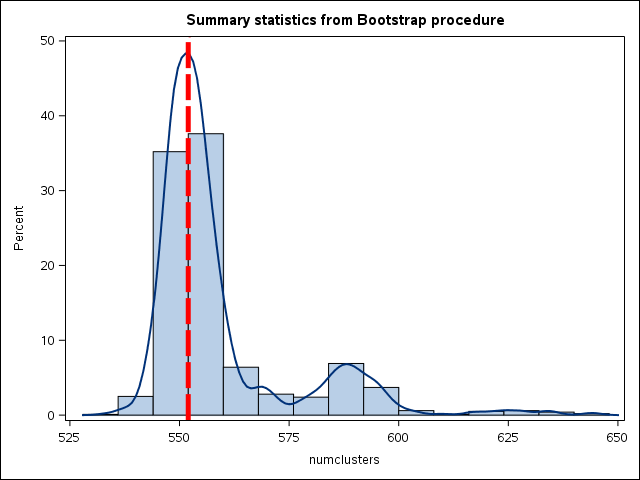
\includegraphics[width=0.33\textwidth]{./figures/numclusters_jtw2009.png}
&
%\caption{Number of Clusters}
%\end{subfigure}
%\begin{subfigure}
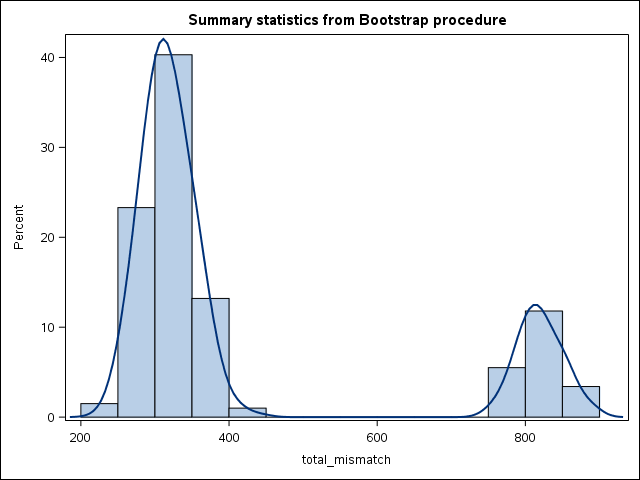
\includegraphics[width=0.33\textwidth]{./figures/mismatchedcounties_jtw2009.png}
\\
{(a) Mean Cluster Size}&
{(b) Number of Clusters}&
%\caption
{(c)Mismatched Counties}
\\
\multicolumn{3}{p{6.2in}}{\footnotesize \emph{Notes:} Histograms plot the density of summary statistics from commuting zones produced using the TS1996 methodology from 1000 simulations of Margins of Error from the 2009-2013 ACS commuting flows data. Red lines provide the summary statistics from commuting zones produced from the published ACS estimates (mean cluster size of 5.63 for 552 clusters).}\\
%\end{subfigure}
\end{tabular}
\label{fig:perturbation}
\end{figure}
\normalsize 


%
We iterate over this procedure 1000 times in order to obtain distributions for these statistics. These graphs are shown in Figure~\ref{fig:perturbation}, where the red vertical dashed lines are the values that would be obtained using only the published figures (without MOE purturbations). Note that there are fewer clusters in the TS1996 implementation for JTW based on ACS, with 551 formed based on the published data compared with 741 in TS1990 and 709 in TS2000.\footnote{We use the same cutoff here as in FKV1990, our replication of TS1990. While commuting flows have increased in distance since 1990 (see Table \ref{tab:comstat}), it is not clear why the same methodology on later data results in so many fewer zones. These results hold irrespective of cluster height.} As one can see, the average cluster size has a wide range of values; while most values are around what the published numbers would give, there is still a substantial portion that have smaller than average clusters. Second, the number of clusters ranges widely, 330 to 450. Finally, the share of population that is mismatched is on average about 5\% of the US population, a small but non-negligible number.
Overall, the underlying measurement error in the data causes uncertainty in the cluster definitions, which is exacerbated by the sharp cutoff imposed in cluster analysis, which we discuss in the next subsection.

\subsection{Distribution of Cluster Height \label{sec:clusterheight}}

We turn to the sensitivty of the clustering to the chosen cutoff value. \citet{TK1987}, describe the algorithm for choosing a cutoff value as follows: ``As a rule of thumb, a normalized average distance of 0.98 was considered sufficient distance between sets of counties to treat them as separate [Labor Market Areas]'' \citep[page 15]{TK1987}.  The article does not provide an analysis of the sensitivity to changing the cutoff marginally up or down. In this subsection, we investigate how sensitive the resultant clusters are to the choice of the cutoff value.


% Source program: /modules/module_clustjtw1990.sas
% Last updated:


%%%%% COMMUTING ZONES
\begin{figure}[th]\centering
\caption{Distribution of Cluster Consolidation, by Height }
\begin{tabular}{c}
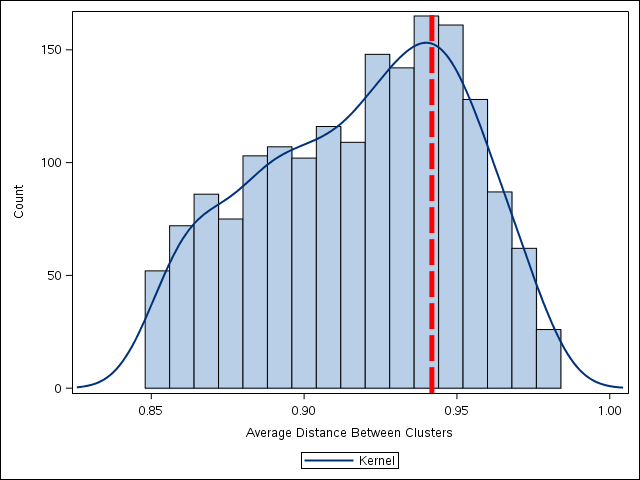
\includegraphics[width=.48\textwidth]{./figures/distancebetweenclusters.png}\\
\multicolumn{1}{p{4in}}{\footnotesize \emph{Notes:} Histograms plot number of
clusters that form at various heights, based on hierarchical clustering
procedure. The vertical line is the value that most closely replicates TS1990.}
\label{fig:heightdensity}
\end{tabular}
\end{figure}



Figure \ref{fig:heightdensity}  show the distribution of heights at which clusters merge using the national 1990 JTW data, with the vertical line indicating the cutoff we chose that most closely approximated TS1996 (0.9418). The key takeaway from this figure is that marginally increasing or decreasing the cutoff causes a substantial number of clusters to be formed or not. In fact, increasing the cutoff to 0.9428 causes the number of clusters to fall by 19, while decreasing the cutoff to 0.9408 causes the number of clusters to increase by 17.\footnote{Another consideration, not discussed here, is that TS1996 normalize the heights within each region before clustering. This causes the cutoff to be at different absolut heights depending on the region.}

As we described above, the measurement error in commuting flows causes some uncertainty in terms of true dissimilarity, and hence true cluster height. Because of the presence of a strict cutoff, some clusters that would have formed (if there were no measurement error) did not form, and vice-versa. More broadly, TS1996 provide no empirical guidance for choosing the `optimal' cutoff and cluster size other than referring to expert knowledge. Later, in Section \ref{sec:objfn}, we consider measures of local labor market integration that may be informative of the optimality of various clustering definitions. 

%\subsection{Other Weaknesses of CZ Methodology}

%In addition to the uncertainty due to data and methodology detailed above, commuting zone construction has a few other features that make it a less than ideal description of local labor markets. First, because the method does not consider the size of counties, the commuting zones in the East half of the country are systematically smaller than the zones on the West half of the country, solely because of the size of the counties. Second, because commuting zones are defined solely based on commuting flows, they do not fully capture local labor market integration; as we noted earlier, these only capture \textit{realized} flows at a point in time, not historical or potential flows. Finally, the clustering method used in TS1996 is very dependent on the order of the first few clusters formed, which makes it more sensitive to error in the data inputs than other clustering methods.	

%First, if we define local labor markets only based on \emph{realized} commuting flows, we overlook other ways in which labor markets are integrated, such as wage levels and unemployment rates. Second, solely using commuting flows is also an issue because they are measured using survey data, and hence are subject to sampling error. This second fact, paired with the strict cutoff, overstates the certainty in the commuting zone defintions.

